\documentclass[11pt]{article}

\usepackage[T1]{fontenc}
\usepackage[utf8]{inputenc}
\usepackage{lmodern}
\usepackage{tikz}

\usepackage{fancyhdr} % Required for custom headers
\usepackage{lastpage} % Required to determine the last page for the footer
\usepackage{extramarks} % Required for headers and footers
\usepackage{graphicx} % Required to insert images
\usepackage{lipsum} % Used for inserting dummy 'Lorem ipsum' text into the template
\usepackage{enumerate}
\usepackage{hyperref}
\usepackage{appendix}
\usepackage{xcolor}

\usepackage{amsmath}
\usepackage{bm}

% Margins
% Esta é uma parte importante, assim mais texto é
% escrito em cada página, as margens aqui estão 
% maiores do que o padrão do latex
\topmargin=-0.45in
\evensidemargin=0in
\oddsidemargin=0in
\textwidth=6.5in
\textheight=9.5in
\headsep=0.25in 

\linespread{1.1} % Line spacing

% Set up the header and footer
\pagestyle{fancy}
\lhead{ataias.github.io} % Top left header
\chead{} % Top center header
\rhead{\firstxmark} % Top right header
\lfoot{\lastxmark} % Bottom left footer
\cfoot{\hmwkTitle} % Bottom center footer
\rfoot{Page\ \thepage\ of\ \pageref{LastPage}} % Bottom right footer
\renewcommand\headrulewidth{0.4pt} % Size of the header rule
\renewcommand\footrulewidth{0.4pt} % Size of the footer rule

\setlength\parindent{0pt} % Removes all indentation from paragraphs

%----------------------------------------------------------------------------------------
%	DETALHES
%----------------------------------------------------------------------------------------

\newcommand{\hmwkTitle}{Solving Poisson Equation with Neumann Conditions} \newcommand{\hmwkSupervisor}{Yuri Dumaresq Sobral} % Teacher/lecturer
\newcommand{\hmwkAuthorName}{Ataias Pereira Reis} % Your name

%----------------------------------------------------------------------------------------
%	TITLE PAGE
%----------------------------------------------------------------------------------------

\title{
\vspace{2in}
\textmd{\textbf{\hmwkTitle}}\\
\vspace{0.1in}\large{Orientador: \textit{\hmwkSupervisor}}
\vspace{3in}
}

\author{\textbf{\hmwkAuthorName}}
\date{} % Insert date here if you want it to appear below your name

\newcommand{\domainOne}[0]{
\begin{center}
\tikzstyle{help lines}+=[dashed]% 
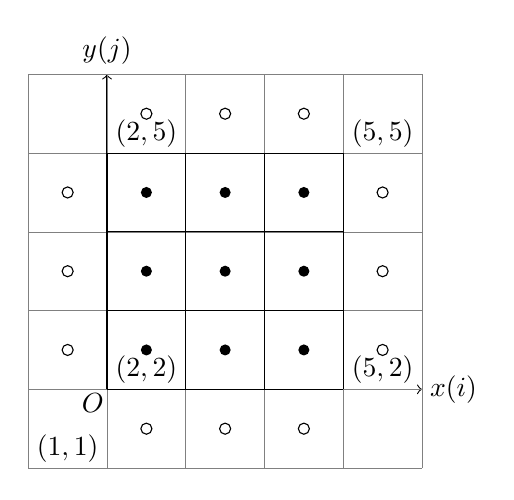
\begin{tikzpicture}
%axes
\draw[->] (0,3) -- (xyz cs:y=4);
\draw (0,4.3) node {$y(j)$};
\draw[->] (3,0) -- (xyz cs:x=4);
\draw (4.4,0) node {$x(i)$};
\draw (-0.18,-0.18) node {$O$};
\draw (-0.5,-0.75) node {$(1,1)$};
\draw (0.5,0.25) node {$(2,2)$};
\draw (3.5,3.25) node {$(5,5)$};
\draw (0.5,3.25) node {$(2,5)$};
\draw (3.5,0.25) node {$(5,2)$};

%grid
\draw[style=help lines] (-1,-1) grid +(5,5);
\draw (0,0) grid +(3,3);
%internal p points
\foreach \x in {0.5,1.5,2.5}
  \foreach \y in {0.5,1.5,2.5}
  {
  \fill (canvas cs:x=\x cm,y=\y cm) circle (2pt);
}
%External p points
\foreach \x in {0.5,1.5,2.5}
  \draw (\x,-0.5) circle (2pt);
\foreach \y in {0.5,1.5,2.5}
  \draw (3.5,\y) circle (2pt);
\foreach \y in {0.5,1.5,2.5}
  \draw (-0.5,\y) circle (2pt);
\foreach \x in {0.5,1.5,2.5}
  \draw (\x,3.5) circle (2pt);

\end{tikzpicture} 
\end{center}}



\begin{document}
\section{Poisson}
\paragraph{} When I started my junior research project, I learned how to solve Poisson with Dirichlet conditions easily using finite differences. It is much faster than the explicit method and the error has the same order as long as you use the same formulas. Feel free to correct me if I am wrong. You may want to know a little of finite differences before proceeding.

\subsection{Grid}
\paragraph{} Before we decide which formulas to use, let's choose a grid. I though the staggered grid would be better as I would get second order central derivative easily for the boundary conditions. I would need a one-sided finite difference formula in the case of a grid where the values are stored in the corners, instead of the center of the cells in the mesh. An example of the grid is available below. We will show the formulas to each of the cells, so it is easier to have a small grid and then you find out an algorithm to create the matrix.
\domainOne

\subsection{Discretization}
\paragraph{} For the discretization, I will use second order finite differences. Let's begin! We want to solve the equation:

\begin{equation}
\nabla^2 u = \frac{\partial^2 u}{\partial x^2} + \frac{\partial^2 u}{\partial y^2} = f(x,y)
\end{equation}

\paragraph{} Let's also consider that in our square grid, $x$ and $y$ vary from 0 to 1, so we have a unit square. Central differences of second order for the partial second derivatives will be used. For an internal point, one has:

\begin{eqnarray}
\frac{u_{i-1j} - 2u_{ij} + u_{i+1j}}{\Delta x^2}	+ \frac{u_{ij-1} - 2u_{ij} + u_{ij+1}}{\Delta x^2} = f_{ij}
\end{eqnarray}


\paragraph{} For the explicit method, you just isolate $u_{ij}$ and iterate. On the other hand, for the implicit method, one has to consider all equations that the system gives you in order to solve it. In this case, one has to solve a problem of the type:

\begin{eqnarray}
Ax = b	
\end{eqnarray}

\paragraph{} Matrix $A$ depends on our discretization and also the boundary conditions if they are of the type Neumann. $b$ is made with values of $f$ and boundary conditions. $x$ is a vector that has all the internal points of the grid. The external points are easy to find once you have the internal ones, you just need to apply the equations for the boundary conditions. Now, for the nine internal points, we have:

\begin{eqnarray}
-4u_{22} + u_{32} + \boldsymbol{u_{12}} + u_{23} + \boldsymbol{u_{21}} &=& \Delta x^2 f_{22}\\
-4u_{23} + u_{33} + \boldsymbol{u_{13}} + u_{24} + u_{22} &=& \Delta x^2 f_{23}\\
-4u_{24} + u_{34} + \boldsymbol{u_{14}} + \boldsymbol{u_{25}} + u_{23} &=& \Delta x^2 f_{24}
\end{eqnarray}


\begin{eqnarray}
-4u_{32} + u_{42} + u_{22} + u_{33} + \boldsymbol{u_{31}} &=& \Delta x^2 f_{32}\\
-4u_{33} + u_{43} + u_{23} + u_{34} + u_{32} &=& \Delta x^2 f_{33}\\
-4u_{34} + u_{44} + u_{24} + \boldsymbol{u_{35}} + u_{33} &=& \Delta x^2 f_{34}
\end{eqnarray}

\begin{eqnarray}
-4u_{42} + \boldsymbol{u_{52}} + u_{32} + u_{43} + \boldsymbol{u_{41}} &=& \Delta x^2 f_{42}\\
-4u_{43} + \boldsymbol{u_{53}} + u_{33} + u_{44} + u_{42} &=& \Delta x^2 f_{43}\\
-4u_{44} + \boldsymbol{u_{54}} + u_{34} + \boldsymbol{u_{45}} + u_{43} &=& \Delta x^2 f_{44}
\end{eqnarray}

\paragraph{} The bold points are boundary points. Notice we have 9 equations, but there are 21 unknown values. What to do now? The rest of the equations are actually defined by boundary conditions. As we have Neumann conditions, those equations define the derivatives on the boundary. We have the following:

\begin{eqnarray}
u_x\left(0, y\right) & = & (u_{2j} - u_{1j})/\Delta x\\
u_x\left(1, y\right) & = & (u_{5j} - u_{4j})/\Delta x\\
u_y\left(x, 0\right) & = & (u_{i2} - u_{i1})/\Delta x\\
u_y\left(x, 0\right) & = & (u_{i5} - u_{i4})/\Delta x
\end{eqnarray}

\paragraph{} From the equations above, we get the twelve equations that the system is missing. Instead of adding it directly as new equations, one could substitute them in the nine equations from before. I will let the substitution to the reader and I will skip for the end matrix system.

\begin{eqnarray}
\left[\begin{array}{ccccccccc}
-2 & 1 & 0 & 1 & 0 & 0 & 0 & 0 & 0\\
1 & -3 & 1 & 0 & 1 & 0 & 0 & 0 & 0\\
0 & 1 & -2 & 0 & 0 & 1 & 0 & 0 & 0\\
1 & 0 & 0 & -3 & 1 & 0 & 1 & 0 & 0\\
0 & 1 & 0 & 1 & -4 & 1 & 0 & 1 & 0\\
0 & 0 & 1 & 0 & 1 & -3 & 0 & 0 & 1\\
0 & 0 & 0 & 1 & 0 & 0 & -2 & 1 & 0\\
0 & 0 & 0 & 0 & 1 & 0 & 1 & -3 & 1\\
0 & 0 & 0 & 0 & 0 & 1 & 0 & 1 & -2 
\end{array}\right] \left[\begin{array}{c}
u_{22}\\ u_{23}\\ u_{24}	\\ u_{32}\\ u_{33}\\ u_{34}\\ u_{42}\\u_{43} \\u_{44}
\end{array}\right] = b
\end{eqnarray}

\begin{eqnarray}
b & = & \Delta x\left[\begin{array}{c}
u_x\left(0, \frac{\Delta x}{2}\right) + u_y\left(\frac{\Delta x}{2},0\right)\\
u_x\left(0, \frac{3\Delta x}{2}\right)\\
u_x\left(0, \frac{5\Delta x}{2}\right) - u_y\left(\frac{\Delta x}{2},1\right)\\
u_y\left(\frac{3\Delta x}{2},0\right)\\
0 \\
-u_y\left(\frac{3\Delta x}{2},1\right)\\
-u_x\left(1, \frac{\Delta x}{2}\right) + u_y\left(\frac{5\Delta x}{2},0\right)\\
-u_x\left(1, \frac{3\Delta x}{2}\right)\\
-u_x\left(1, \frac{5\Delta x}{2}\right) - u_y\left(\frac{5\Delta x}{2}, 1\right)
\end{array}\right] + \Delta x^2 \left[\begin{array}{c}
f_{22}\\ f_{23}\\ f_{24}	\\ f_{32}\\ f_{33}\\ f_{34}\\ f_{42}\\f_{43} \\f_{44}
\end{array}\right]
\end{eqnarray}

\paragraph{} Before implementing that, let's take a look at $A$'s eigenvalues:

\begin{eqnarray}
\left[ -6, -4, -4, -3, -3, -2, -1, -1, -2.5327\times 10^{-16}\right]
\end{eqnarray}

\paragraph{} Those values were obtained with the aid of a computer. Well, the last value seems like 0. It the eigenvalue of a matrix is 0, it doesn't have an inverse so we can't use it to solve a linear system. Well, what about pseudo-inverse? I thought of that, but I haven't tried it. What does this eigenvalue of zero mean? Well, it means that you have one degree of freedom. You can actually pick a point to be what you want and then solve it. I want the gradient of the function only, for my problem of Navier Stokes. Maybe you want a function with mean 0 for your purposes... or whatever, you can just select a point to the value you want and check if the matrix will be invertible. Choose one of the boundaries. I chose $u_{12} = 0$. The only modifications are:

\begin{eqnarray}
A[1,1] &=& -3\\
b[1] & = & u_y\left(\frac{\Delta x}{2},0\right)\Delta x + \Delta x^2 f_{22}
\end{eqnarray}

\paragraph{} You can make an algorithm for that. I have made one as well, I wrote it in Julia language.\footnote{Code available at: \url{https://gist.github.com/ataias/05ebdad6dfc6ee56e44f}}

\paragraph{} Any suggestions, feel free to contact me through the gist or at ataiasreis at gmail. 
\end{document}


